% Created 2022-08-14 dom 18:12
% Intended LaTeX compiler: pdflatex
\documentclass[11pt]{article}
\usepackage[utf8x]{inputenc}
\usepackage[T1]{fontenc}
\usepackage{graphicx}
\usepackage{grffile}
\usepackage{longtable}
\usepackage{wrapfig}
\usepackage{rotating}
\usepackage[normalem]{ulem}
\usepackage{amsmath}
\usepackage{textcomp}
\usepackage{amssymb}
\usepackage{capt-of}
\usepackage{hyperref}
\author{José A. Alonso}
\date{\today}
\title{}
\hypersetup{
 pdfauthor={José A. Alonso},
 pdftitle={},
 pdfkeywords={},
 pdfsubject={},
 pdfcreator={Emacs 27.1 (Org mode 9.4.6)},
 pdflang={Spanish}}
\begin{document}

\tableofcontents


\section{1° de Bachillerato (16 años)}
\label{sec:org5ed31f5}

Del libro \href{http://www.apuntesmareaverde.org.es/grupos/mat/LOMLOE/Bachillerato/Matematicas\_I.pdf}{Matemáticas I (1º de Bachillerato)} de Apuntes marea Verde.

\subsection{Números reales y complejos}
\label{sec:org13d0810}

\subsubsection{Valor absoluto}
\label{sec:org6bb0a22}

\begin{itemize}
\item 10 No negatividad: \(|a| \geq 0\).

\item 10
\begin{teorema}
Simetría: \(|a| = |-a|\).
\end{teorema}
\begin{demostracion}
Si \(a > 0\), entonces
\begin{align*}
|a| &= a \\
    &= -(-a) \\
    &= |-a|
\end{align*}

Si \(a = 0\), entonces
\begin{align*}
    |a| &= |0| \\
        &= |-0| \\
        &= |-a|
\end{align*}

Si \(a < 0\), entonces
\begin{align*}
|a| &= -a \\
    &= |-a|
\end{align*}
\end{demostracion}

\item 10 Definición positiva: Si \(|a| = 0\), entonces \(a = 0\).

\item 10 Valor absoluto y producto: \(|a \times b| = |a| \times |b|\).

\item 10 Desigualdad triangular: \(|a + b| \leq |a| + |b|\).
\end{itemize}

\subsubsection{Distancia en la recta real}
\label{sec:org68e0f9f}

\begin{itemize}
\item 12 La distancia está definida por \(\mbox{dist}(x,y) = |x - y|\) y
verifica las siguientes propiedades:
\begin{itemize}
\item \(\mbox{dist}(x,y) = 0\) syss \(x = y\)
\item \(\mbox{dist}(x,y) = \mbox{dist}(y,x)\)
\item \(\mbox{dist}(x,y) \leq \mbox{dist}(x,z) + \mbox{dist}(z,y)\)
\end{itemize}
\end{itemize}

\subsubsection{Números complejos}
\label{sec:org0b88f70}

\begin{itemize}
\item 21 Operaciones en forma binómica:
\begin{itemize}
\item \((x + iy) + (u + iv) = (x + u) + i(y + v)\).
\item \((x + iy) (u + iv) = (xu - yv) + i(xv + yu)\).
\end{itemize}

\item 27 Propiedades del módulo, del conjugado y del argumento de un número
complejo:
\begin{itemize}
\item \(\overline{z+w} = \overline{z} + \overline{w}\)
\item \(\overline{z-w} = \overline{z} - \overline{w}\)
\item \(\overline{z \cdot w} = \overline{z} \cdot \overline{w}\).
\item \(\arg({\overline{z}}) = -\arg({z})\).
\item \(z \in \mathbb{R} \iff z = \overline{z}\).
\item \(z \cdot \overline{z} = |z|^{2}\)
\item \(|\overline{z}| = |z|\).
\item \(|z \cdot w| = |z| \cdot |w|\)
\item \(\left|\dfrac{z}{w}\right| = \dfrac{|z|}{|w|}\)
\item \(|z| = 0 \iff z = 0\)
\item \(\Re(z) = \dfrac{z + \overline{z}}{2}\)
\item \(\Im(z) = \dfrac{z - \overline{z}}{2i}\)
\item \(\Re(z) \leq |z|\)
\item \(\Im(z) \leq |z|\)
\item \(|z| \leq \Re(z) + \Im(z)\)
\item \(||z| - |w|| \leq |z + w| \leq |z| + |w|\)
\end{itemize}
\end{itemize}

\subsubsection{Operaciones entre números complejos en forma trigonométrica}
\label{sec:org029e8f9}

\begin{itemize}
\item 29
\begin{teorema}
Para multiplicar números complejos expresados en forma polar o en
trigonométrica basta multiplicar sus módulos y sumar sus argumento
\end{teorema}
\begin{demostracion}
\begin{align*}
z_{} \cdot z' &= r_{}(\cos \alpha + i\sen \alpha) \cdot r'(\cos \beta + i \sen \beta)  \\
       &= (r \cdot r') ((\cos \alpha \cos \beta - \sen \alpha \sen \beta) + i (\sen \alpha \cos \beta - \cos \alpha \sen \beta))   \\
       &= (r \cdot r') (\cos (\alpha + \beta) + i \sen (\alpha + \beta))  \\
\end{align*}
\end{demostracion}

\item Para dividir números complejos, basta dividir sus módulos y restar
sus argumentos.

\item El inverso de un número complejo distinto de cero tiene como módulo,
el inverso del módulo, y como argumento, el opuesto del argumento.

\item Para elevar un número complejo a una potencia, se eleva el módulo a
dicha potencia, y se multiplica el argumento por el exponente.
\end{itemize}

\subsection{Trigonometría}
\label{sec:org2cec6d5}

\subsubsection{Razones trigonométricas de la suma de ángulos}
\label{sec:orgcd5c4a4}

\begin{itemize}
\item 116 \(\sen(a + b) = \sen(a)\cos(b) + \cos(a)\sen(b)\)

\item 116 \(\cos(a + b) = \cos(a)\cos(b) - \sen(a)\sen(b)\)

\item 117
\begin{teorema}
\(\tan(a+b) = \dfrac{\tan(a)+\tan(b)}{1-\tan(a)\tan(b)}\)
\end{teorema}
\begin{demostracion}
\begin{align*}
\tan(a+b) &= \dfrac{\sen(a+b)}{\cos(a+b)} \\
          &= \dfrac{\sen(a)\cos(b)+\cos(a)\sen(b)}
                   {\cos(a)\cos(b)-\sen(a)\sen(b)} \\
          &= \dfrac{\dfrac{\sen(a)\cos(b)+\cos(a)\sen(b)}{\cos(a)\cos(b)}}
                   {\dfrac{\cos(a)\cos(b)-\sen(a)\sen(b)}{\cos(a)\cos(b)}} \\
          &= \dfrac{\tan(a)+\tan(b)}{1-\tan(a)\tan(b)} \\
\end{align*}
\end{demostracion}
\end{itemize}

\subsubsection{Razones trigonométricas de la resta de ángulos}
\label{sec:org9acae32}

\begin{itemize}
\item 117 \(\sen(-a) = -\sen(a)\)

\item 117 \(\cos(-a) = \cos(a)\)

\item 117 \(\tan(-a) = -\tan(a)\)

\item 118 \(\sen(a-b) = \sen(a)\cos(b) - \cos(a)\sen(b)\)

\item 118 \(\cos(a-b) = \cos(a)\cos(b) + \sen(a)\sen(b)\)

\item 118 \(\tan(a-b) = \dfrac{\tan(a) - \tan(b)}{1 + \tan(a)\tan(b)}\)
\end{itemize}

\subsubsection{Razones trigonométricas del ángulo doble}
\label{sec:org898db59}

\begin{itemize}
\item 118 \(\sen(2a) = 2\sen(a)\cos(a)\)

\item 118 \(\cos(2a) = \cos^{2}(a) - \sen^2(a)\)

\item 118 \(\tan(2a) = \dfrac{2\tan(a)}{1 - \tan^{2}(a)}\)

\item 119 \(\sen\left(\dfrac{a}{2}\right) = \pm\sqrt{\dfrac{1-\cos(a)}{2}}\)
\end{itemize}


\begin{itemize}
\item 119 \(\cos\left(\dfrac{a}{2}\right) = \pm\sqrt{\dfrac{1+\cos(a)}{2}}\)
\end{itemize}


\begin{itemize}
\item 119 \(\tan\left(\dfrac{a}{2}\right) = \pm\sqrt{\dfrac{1-\cos(a)}{1+\cos(a)}}\)
\end{itemize}

\subsubsection{Transformaciones de sumas de razones trigonométricas en productos}
\label{sec:org26dd84b}

\begin{itemize}
\item Fórmula de Simpson de seno por coseno: \\
\begin{teorema}
\(\sen \alpha \cos \beta = \dfrac{\sen(\alpha+\beta) + \sen(\alpha-\beta)}{2}\)
\end{teorema}
\begin{demostracion}
(en ProofWiki \href{https://proofwiki.org/wiki/Simpson\%27s\_Formulas/Sine\_by\_Cosine}{Simpson's formulas/Sine by cosine})

\begin{align*}
 &  \dfrac{\sen(\alpha+\beta) + \sen(\alpha-\beta)}{2} \\
 &= \dfrac{(\sen \alpha \cos \beta + \cos \alpha \sen \beta) + (\sen \alpha \cos \beta - \cos \alpha \sen \beta)}{2} \\
 &= \dfrac{2 \sen \alpha \cos \beta}{2} \\
 &= \sen \alpha \cos \beta
\end{align*}
\end{demostracion}

\item 120
\begin{teorema}
\(\sen(a) + \sen(b) =
  2\sen\left(\dfrac{a+b}{2}\right)\cos\left(\dfrac{a-b}{2}\right)\)
\end{teorema}
\begin{demostracion}
(En ProofWiki \href{https://proofwiki.org/wiki/Prosthaphaeresis\_Formulas/Sine\_plus\_Sine}{Prosthaphaeresis formulas/Sine plus sine}).

\begin{align*}
  &  2 \sen\left(\dfrac{\alpha+\beta}{2}\right)
       \cos\left(\dfrac{\alpha-\beta}{2}\right) \\
  &= 2 \dfrac{\sen\left(\dfrac{\alpha+\beta}{2} + \dfrac{\alpha-\beta}{2}\right) +
              \sen\left(\dfrac{\alpha+\beta}{2} - \dfrac{\alpha-\beta}{2}\right)}
             {2}
       & \mbox{Fórmula de Simpson} \\
  &= \sen \frac{2\alpha}{2} + \sen \frac{2\beta}{2} \\
  &= \sen \alpha + \sen \beta \\
\end{align*}
\end{demostracion}

\item 120
\begin{teorema}
\(\sen(a) - \sen(b) =
  2\cos\left(\dfrac{a+b}{2}\right)\sen\left(\dfrac{a-b}{2}\right)\)
\end{teorema}
\begin{demostracion}
(en ProofWiki \href{https://proofwiki.org/wiki/Prosthaphaeresis\_Formulas/Sine\_minus\_Sine}{Prosthaphaeresis formulas/sine minus sine})

\begin{align*}
  &  2 \cos\left(\dfrac{\alpha+\beta}{2}\right)
       \sen\left(\dfrac{\alpha-\beta}{2}\right) \\
  &= 2 \dfrac{\sen\left(\dfrac{\alpha-\beta}{2} + \dfrac{\alpha+\beta}{2}\right) +
              \sen\left(\dfrac{\alpha-\beta}{2} - \dfrac{\alpha+\beta}{2}\right)}
             {2}
       & \mbox{Fórmula de Simpson} \\
  &= \sen \frac{2\alpha}{2} - \sen \frac{2\beta}{2} \\
  &= \sen \alpha - \sen \beta \\
\end{align*}
\end{demostracion}

\item Fórmula de Simpson de coseno por coseno: \\
\begin{teorema}
\(\cos \alpha \cos \beta = \dfrac{\cos(\alpha-\beta) + \cos(\alpha+\beta)}{2}\)
\end{teorema}
\begin{demostracion}
(en ProofWiki \href{https://proofwiki.org/wiki/Simpson\%27s\_Formulas/Cosine\_by\_Cosine}{Simpson's Formulas/Cosine by Cosine})

\begin{align*}
 &  \dfrac{\cos(\alpha-\beta) + \sen(\alpha+\beta)}{2} \\
 &= \dfrac{(\cos \alpha \cos \beta + \sen \alpha \sen \beta) + (\cos \alpha \cos \beta - \sen \alpha \sen \beta)}{2} \\
 &= \dfrac{2 \cos \alpha \cos \beta}{2} \\
 &= \cos \alpha \cos \beta
\end{align*}
\end{demostracion}

\item 120
\begin{teorema}
\(\cos a  + \cos b  =
  2\cos\left(\dfrac{a+b}{2}\right)\cos\left(\dfrac{a-b}{2}\right)\)
\end{teorema}
\begin{demostracion}
(en ProofWiki \href{https://proofwiki.org/wiki/Prosthaphaeresis\_Formulas/Cosine\_plus\_Cosine}{Prosthaphaeresis Formulas/Cosine plus Cosine}).

\begin{align*}
  &  2 \cos\left(\dfrac{\alpha+\beta}{2}\right)
       \cos\left(\dfrac{\alpha-\beta}{2}\right) \\
  &= 2 \dfrac{\cos\left(\dfrac{\alpha-\beta}{2} - \dfrac{\alpha-\beta}{2}\right) +
              \cos\left(\dfrac{\alpha+\beta}{2} + \dfrac{\alpha-\beta}{2}\right)}
             {2}
       & \mbox{Fórmula de Simpson} \\
  &= \cos \frac{2\beta}{2} + \cos \frac{2\alpha}{2} \\
  &= \cos \alpha + \cos \beta \\
\end{align*}
\end{demostracion}

\begin{itemize}
\item 120
\end{itemize}
\begin{teorema}
\(\cos a  - \cos b  =
  -2\sen\left(\dfrac{a+b}{2}\right)\sen\left(\dfrac{a-b}{2}\right)\)
\end{teorema}
\begin{demostracion}
(en ProofWiki \href{https://proofwiki.org/wiki/Prosthaphaeresis\_Formulas/Cosine\_minus\_Cosine}{Prosthaphaeresis Formulas/Cosine minus Cosine}).

\begin{align*}
  &  -2 \sen\left(\dfrac{\alpha+\beta}{2}\right)
        \sen\left(\dfrac{\alpha-\beta}{2}\right) \\
  &= -2 \dfrac{\cos\left(\dfrac{\alpha+\beta}{2} - \dfrac{\alpha-\beta}{2}\right) -
               \cos\left(\dfrac{\alpha+\beta}{2} + \dfrac{\alpha-\beta}{2}\right)}
             {2}
       & \mbox{Fórmula de Simpson} \\
  &= -\left(\cos \frac{2\beta}{2} - \cos \frac{2\alpha}{2}\right) \\
  &= \cos \alpha - \cos \beta \\
\end{align*}
\end{demostracion}
\end{itemize}

\subsubsection{Resolución general de triángulos}
\label{sec:orgc13c1d7}

\begin{itemize}
\item 129
\begin{teorema}
Teorema del coseno: Sea \(\triangle ABC\) un triángulos cuyos lados
\(a, b, c\) son tales que \(a\) es opuesto de \(A\), \(b\) es opuestos de \(B\)
y \(c\) es opuesto de \(C\). Entonces,
$$c^2 = a^2 + b^2 - 2 a b \cos C$$
\end{teorema}
\begin{demostracion}
(En ProofWiki \href{https://proofwiki.org/wiki/Law\_of\_Cosines}{Law of cosines}).

\emph{Caso de triángulo rectángulo}

Sea \(\triangle ABC\) un triángulo rectángulo tal que \(\angle A\) recto.

\begin{center}
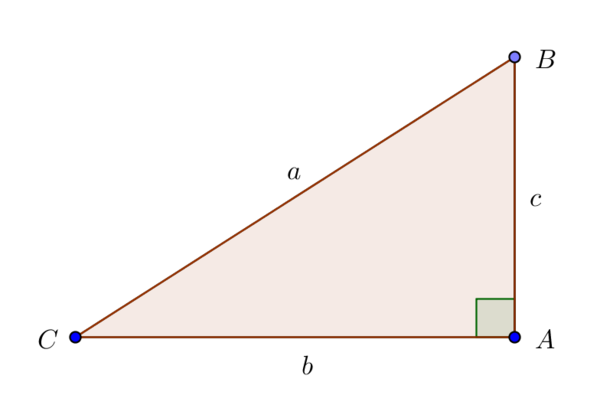
\includegraphics[width=.9\linewidth]{./fig/teorema-coseno-1.png}
\end{center}

\begin{align*}
a^2 &= b^2 + c^2
    && \text{Teorema de Pitágoras} \\
c^2 &= a^2 - b^2
    && \text{Despejando $c^{2}$}\\
    &= a^2 - 2 b^2 + b^2
    && \text{Sumando $0 = b^2 - b^2$ a la derecha} \\
    &= a^2 - 2 a b \left({\frac b a}\right) + b^2
    && \text{Multiplicando $2 b^2$ por $\dfrac a a$} \\
    &= a^2 + b^2 - 2 a b \cos C
    && \text{Por la definición de $\cos C = \dfrac b a$}
\end{align*}


\emph{Caso del triángulo acutángulo}

Sea \(\triangle ABC\) un triángulo acutángulo.

\begin{center}
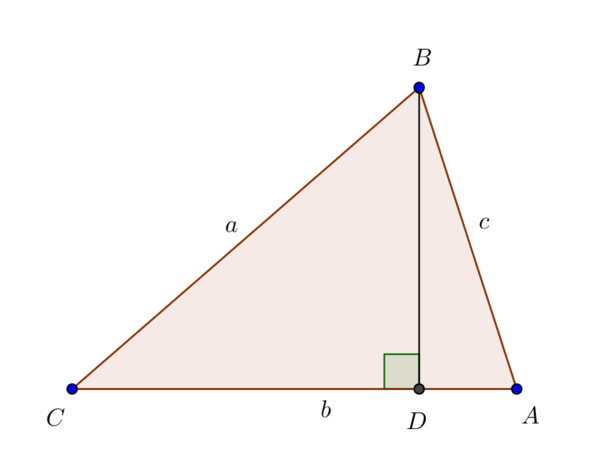
\includegraphics[width=.9\linewidth]{./fig/teorema-coseno.2.png}
\end{center}

Sea \(BD\) perpendicular a \(AC\) y se definen \(h = BD\), \(e = CD\) y \(f = AD\).

Los triángulos \(\triangle CDB\) y \(\triangle ADB\) son rectángulos. Por tanto, \\
\begin{align*}
c^2 &= h^2 + f^2
    && \text{Teorema de Pitágoras} \\
    &= a^2 - e^2 + f^2
    && \text{Teorema de Pitágoras} \\
    &= a^2 - e^2 + f^2 + 2e^2 - 2e^2 + 2ef - 2ef
    && \text{Sumando $2e^2 - 2e^2 + 2ef - 2ef$} \\
    &= a^2 + (e^2 + f^2 + 2ef) - 2e(e + f)
    && \text{Agrupando} \\
    &= a^2 + (e + f)^2 - 2e(e+f)
    && \text{Cuadrado del binomio} \\
    &= a^2 + b^2 - 2eb
    && \text{Sustituyendo $b = e + f$} \\
    &= a^2 + b^2 - 2 a b \cos C
    && \text{Definición de $\cos C = \frac{e}{a}$} \\
\end{align*}

\emph{Caso del triángulo obtusángulo}

Sea \(\triangle ABC\) un triángulo obtusángulo.

\begin{center}
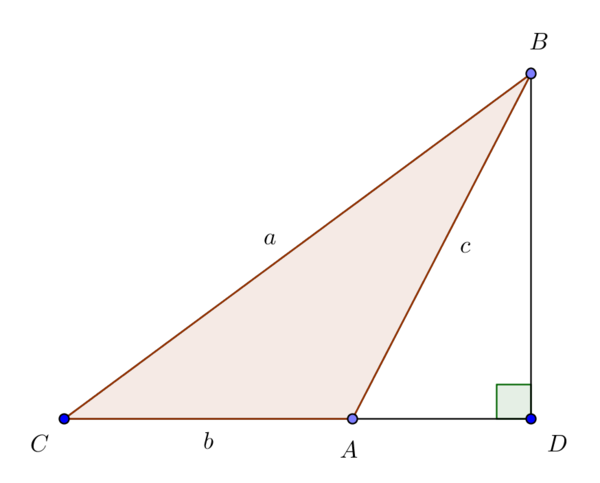
\includegraphics[width=.9\linewidth]{./fig/teorema-coseno-3.png}
\end{center}

Se extiende \(AC\) y sea \(BD\) perpendicular a \(AC\). Se define \(h = BD\), \(e = CD\) y \(f = AD\).

Entonces \(\triangle CDB\) y \(\triangle ADB\) son triángulos rectángulos. Por tanto,

  \begin{align*}
c^2 &= h^2 + f^2
    && \text{Teorema de Pitágoras} \\
    &= a^2 - e^2 + f^2
    && \text{Teorema de Pitágoras} \\
    &= a^2 - (b + f)^2 + f^2
    && \text{Por definición de $e$ y $f$} \\
    &= a^2 - b^2 - f^2 - 2bf + f^2
    && \text{Expandiendo el cuadrado del binomio} \\
    &= a^2 - b^2 - 2bf
    && \text{Cancelando $f^2 - f^2$} \\
    &= a^2 - b^2 - 2bf + 2b^2 - 2b^2
    && \text{Sumando y restando $2b^2$} \\
    &= a^2 + b^2 - 2b(b + f)
    && \text{Reagrupando} \\
    &= a^2 + b^2 - 2be \\
    &= a^2 + b^2 - 2 a b \cos C
    && \text{Por definición de $\cos C = \frac{e}{a}$}
  \end{align*}
\end{demostracion}

\item 129
\begin{teorema}
Teorema de Pitágoras: Sea \(\triangle ABC\) un triángulo rectángulo
\(c\) como su hipotenusa. Entonces,
$$a^2 + b^2 = c^2$$
\end{teorema}
\begin{demostracion}
\begin{align*}
c^2 &= a^2 + b^2 - 2 a b \cos\left(\frac{\pi}{2}\right) \\
    &= a^2 + b^2
\end{align*}
\end{demostracion}
\end{itemize}
\end{document}
